\section{Quantum chromodynamics and low-energy effective theories}\label{sec:qcdModels}
At his point we want to give a brief overview and introduction into \acrrepeat{qcd} as the established fundamental, microscopic theory of the strong interaction.
The purpose of this introduction is to facilitate the introduction of the \acrrepeat{qm} model as a natural \loeft{} of \qcd{}, in \cref{subsec:chiralLEFT}.
In this work we are mainly focused on chiral symmetry and its spontaneous breaking and subsequent restoration at non-zero temperature and quark chemical potential by quantum and thermodynamic fluctuations.

A complete and self-contained introduction to \qcd{} in general and in the context of \frg{} is far beyond the scope of this work. 
For a more detailed discussion, we refer to, \eg{}, the textbooks~\cite{Ryder1996Jun,Peskin:1995ev,Burgess2006Dec,Greiner2007,Schwartz2013Dec} and \ccite{Pawlowski:2005xe,Rosten:2010vm,Gies:2006wv,Braun:2014ata,Alkofer:2018guy,PawlowskiQCD,Leonhardt:2019mpy,Dupuis:2020fhh,Gao:2020qsj,Wink:2020tnu,PawlowskiScript,FuQCDRev,FuQCD,Fu4qQCD,} in the context of \frg{}.

This section has a corresponding digital auxiliary file~\cite{Steil:2023PhDqcd}, which includes some computations and plots for the \acrshort{pcac} relation \eqref{eq:PCAC} and the running coupling in \cref{eq:alphagRunning} of \cref{subsec:aFcSB}.
Furthermore it includes the diagrammatic expressions \eqref{eq:QCDUflowDiag}, \eqref{eq:qcd4fermiFlow}, and \eqref{eq:qcd4fermiFlowHad} of \cref{subsec:chiralLEFT}, making use of the functionalities of our \WAM{} code~\cite{Steil:2023PhDFlowEquationsNB}.

\subsection{Quantum chromodynamics}\label{subsec:qcd}
\qcd{} is a non-Abelian gauge theory of massive, spin-$\frac{1}{2}$ fermions called quarks, which exist in $N_f=6$ distinct flavors – up, down, strange, charm, bottom, and top – and each flavor can come in one of $N_c=3$ colors \dash{} refereed to as red, green, and blue in loose analogy to the colors perceived by humans.
In \qcd{}, the gauge group $SU(N_c)=SU(3)$ is obtained by promoting the color charge to a local symmetry. 
The massless, spin-$1$ gauge bosons of \qcd{} are called gluons and mediate the strong interaction of quarks as color charged quanta of the gauge field.
A major difference between \qcd{}, as a non-Abelian \SU{3} gauge theory, and an Abelian gauge theory, like \qed{}, which has an $U(1)$ gauge symmetry, is that gluons in \qcd{} carry color charge.
This allows them to interact not only with quarks but also among themselves, in stark contrast to photons in \qed{}, which carry no electric charge and hence cannot self-interact.
Masses and quantum numbers for quarks and gluons can be found in \cref{tab:quarksandgluons} and will be explained further in the following.

\begin{table}[t]
	\centering
	\caption{\label{tab:quarksandgluons}%
		Properties and quantum numbers of the quarks and gluons of \qcd{}, see, \eg{}, Chap. \textit{15. Quark Model} of \ccite{ParticleDataGroup2022Aug} for additional details.
		The values for the masses $M$ with their experimental uncertainties are from \ccite{ParticleDataGroup2022Aug}.
		Details regarding the definition and potential renormalization (mass-independent subtraction scheme, \viz{} ${\overline{\mathrm{MS}}}$) of the different masses are included in \ccite{ParticleDataGroup2022Aug}.
		The listed quantum numbers are spin $S$, baryon number $B$, electric charge $Q$ in units of the elementary charge $e$, the third-/$z$-component of the isospin $I_3$, and 
		$I(J^P)$ \dash{} isospin $I$, total angular momentum $J$ (here for elementary particles equal to their spin: $J=S$), and conventional, intrinsic parity $P$.
		The quarks have corresponding anti-quarks with identical masses and spins but otherwise quantum numbers of opposite sign and they carry anti-colors in $\bar{\mathbf{3}}$.
		The gluons are considered to be massless in \qcd{} but experimentally \textit{``A mass as large as a few MeV may not be precluded''}~\cite{ParticleDataGroup2022Aug,Yndurain1995Feb}.
	}% Why the protect: [https://tex.stackexchange.com/a/12699/].
	\vspace{\TableAbovecaptionskip}
	\renewcommand{\arraystretch}{1.15}
	\begin{tabular}{l c | r | c c c c c | c}
		\toprule
			Name & Symbol & $M\,(\MeV/c^2)$ & $S$ & $B$ & $Q\,(e)$ & $I_3$ & $I(J^P)$ & colors in\\
			\midrule
			up & u & $2.16_{-0.26}^{+0.49}$ & $\tfrac{1}{2}$ & $\tfrac{1}{3}$ & $+\tfrac{2}{3}$ & $+\tfrac{1}{2}$& $\tfrac{1}{2}\big(\tfrac{1}{2}^+\big)$ & $\mathbf{3}$\\[.1em]
			down & d & $4.67_{-0.17}^{+0.48}$ & $\tfrac{1}{2}$ & $\tfrac{1}{3}$ & $-\tfrac{1}{3}$ & $-\tfrac{1}{2}$ & $\tfrac{1}{2}\big(\tfrac{1}{2}^+\big)$ & $\mathbf{3}$\\[.3em]
			strange & s & $93.4_{-3.4}^{+8.6}$ & $\tfrac{1}{2}$ & $\tfrac{1}{3}$ & $-\tfrac{1}{3}$ & $0$ & $0\big(\tfrac{1}{2}^+\big)$ & $\mathbf{3}$\\[.1em]
			charm & c & $1270_{-20}^{+20}$ & $\tfrac{1}{2}$ & $\tfrac{1}{3}$ & $+\tfrac{2}{3}$ & $0$ & $0\big(\tfrac{1}{2}^+\big)$ & $\mathbf{3}$\\[.3em]
			bottom & b & $4180_{-20}^{+30}$ & $\tfrac{1}{2}$ & $\tfrac{1}{3}$ & $-\tfrac{1}{3}$ & $0$ & $0\big(\tfrac{1}{2}^+\big)$ & $\mathbf{3}$\\[.1em]
			top & t & $172,\mkern-1mu690_{-300}^{+300}	$ & $\tfrac{1}{2}$ & $\tfrac{1}{3}$ & $+\tfrac{2}{3}$ & $0$ & $0\big(\tfrac{1}{2}^+\big)$ & $\mathbf{3}$\\[.1em]
			\midrule
			gluon & g & $0$ & $1$ & $0$ & $0$ & $0$& $0\big(1^-\big)$ & $\mathbf{8}$\\
		\bottomrule
	\end{tabular}
\end{table}

\paragraph{Quarks, gluons, six flavors, and three colors}\phantomsection\label{paragraph:qcdHistory}\mbox{}\\%
Historically quarks as elementary particles were first introduced as part of the \textit{quark model} devised by Murray Gell-Mann~\cite{Gell-Mann:1962yej} and George Zweig~\cite{Zweig:1964ruk,Zweig:1964jf}, see, \eg{}, Chap. \textit{15. Quark Model} of \ccite{ParticleDataGroup2022Aug} for additional details, to explain the large number of diverse hadrons being discovered in maturing collider experiments in the 1950s and continuing through the 1960s.
The preceding organization scheme \dash{} the \textit{``Eightfold Way''}  \dash{} to classify hadrons by Murray Gell-Mann~\cite{GellMann:1961ky} and Yuval Ne’eman~\cite{Neeman1961Aug} follows naturally from the quark model.
The original quark model introduces a \SU{3} flavor symmetry by postulating that hadrons are composed of three types \dash{} flavors \dash{} of quarks: up, down, and strange.
Mesons are understood as quark-anti-quark bound states by coupling quarks in the fundamental representation $\mathbf{3}$ of flavor \SU{3} with anti-quarks in the complex conjugate representation $\mathbf{\bar{3}}$ to form a nonet of meson.
The latter can be decomposed into a singlet in trivial representation $\mathbf{1}$  and an octet in adjoint representation $\mathbf{8}$, \ie{}, $\mathbf{3}\otimes\mathbf{\bar{3}}=\mathbf{8}\oplus\mathbf{1}$.
Baryons are understood as bound states of three quarks.

In the early days of the quark model it was soon realized, first by Oscar W. Greenberg~\cite{Greenberg1964Nov}, that the construction of the antisymmetric wave function required by the Pauli exclusion principle/spin-statistic theorem~\cite{Pauli1925Feb,Pauli1925Feb2,Pauli1940Oct} was problematic for certain baryons, like the spin $S=\frac{3}{2}$ baryon $\Delta^{++}$.
Nine months later, Moo-Young Han and Yoichiro Nambu suggested the existence of a hidden degree of freedom~\cite{Han1965Aug}, which they originally called \SU{3}' \dash{} from a modern point of view the concept of three colors was born.
It took a few years until 1972 when William Bardeen, Harald Fritzsch, and Murray Gell-Mann~\cite{Bardeen:1972xk} established color as the charge of the strong force, which completely commutes with all other charges.
At this point it was possible to understand and construct the antisymmetric wave function of baryons as fully antisymmetric in color and symmetric in the combination of flavor, spin, and space, allowing for a decomposition in flavor as $\mathbf{3}\otimes\mathbf{3}\otimes\mathbf{3}=\mathbf{10}_S\oplus\mathbf{8}_M\oplus\mathbf{8}_M\oplus\mathbf{1}_A$.
This allows for a classification of spin-$\frac{3}{2}$ baryons (like, \eg{}, Delta resonances ${\Delta^{++},\ldots,\Delta^{-}}$) in the flavor symmetric decuplet $\mathbf{10}_S$. 
Light spin-$\frac{1}{2}$ baryons (most notably protons and neutrons) and heavy spin-$\frac{1}{2}$ baryons (excited states or resonances, like, \eg{}, the Roper resonance ${N(1440)1/2^+}$) are mixtures of both octets $\mathbf{8}_M$ with mixed flavour symmetry.

Those developments were driven and in some cases verified by a multitude of high-energy particle physics experiments, see, \eg{}, \ccite{Saito2004Jul} for a review of deep inelastic scattering experiments and \ccite{Brandelik1979Sep,Ellis1979Feb,Brandelik1980Dec,Berger1980Dec,Alexander1991Dec} for information on three-jet events, which in conjunction with aforementioned theoretical advances established the up, down, and strange quark as fundamental particles and the gluon as mediator of the strong force.
Recent experimental data~\cite{ParticleDataGroup2022Aug} put the masses of the three ``light'' flavors up, down, and strange at $m_u\approx2\,\MeV$, $m_d\approx 5\,\MeV$, and $m_s\approx 93\, \MeV$, \cf{} \cref{tab:quarksandgluons}.

Today the quark model and \qcd{} also include the three heavy quark flavors.
The charm quark ($m_c\approx 1.27\, \GeV$~\cite{ParticleDataGroup2022Aug}) was theorized by James Bjorken and Sheldon Glashow~\cite{Bjorken1964Aug} (1964) and Sheldon Glashow, John Iliopoulos, and Luciano Maiani~\cite{Glashow1970Oct} (1970) and experimentally discovered with the $J/\psi$ meson by Samuel Ting \etal{}~\cite{Aubert1974Dec} (1974) at BNL and Burton Richter \etal{}~\cite{Augustin1974Dec} (1974) at SLAC.
The third generation of bottom ($m_b\approx 4.18\, \GeV$~\cite{ParticleDataGroup2022Aug}) and top ($m_t\approx 172.69\, \GeV$~\cite{ParticleDataGroup2022Aug}) heavy quark flavors was theorized by Makoto Kobayashi and Toshihide Maskawa~\cite{Kobayashi1973Feb} (1973).
The bottom quark was experimentally discovered by Leon M. Lederman \etal{}~\cite{Herb1977Aug} (1977) at Fermilab and the top quark was experimentally discovered by the CDF~\cite{CDFCollaboration1995Apr} and D\O{}~\cite{D0Collaboration1995Apr} collaborations (1995).
Quantum numbers for the heavy quarks are listed in \cref{tab:quarksandgluons}.

\paragraph{The classical action of QCD}\phantomsection\label{paragraph:qcdS}\mbox{}\\%
\qcd{} as a \qft{}, as we would recognize it today, was developed by Harald Fritzsch, Heinrich Leutwyler, and Murray Gell-Mann~\cite{Fritzsch1973Nov} in 1973 using the gauge theory developed by Chen Ning Yang and Robert Mills~\cite{Yang:1954ek} (1954) \dash{} the special case of a \SU{3} \ym{} theory, see also \ccite{Mills1989Jun}.
In the following we want to give a brief overview of \qcd{} as a \qft{}.\bigskip

The classical action of \qcd{} in Euclidean space-time is given by
\begin{align}
S_\mathrm{QCD}^0[\FA,\Fpsi,\Fpsib]\equiv \int_x\, \bigg(
\frac{1}{4} F_{\mu\nu}^a F_{\mu\nu}^a
+\Fpsib(\gamma_\mu D_\mu +\hat{m}- \gamma_4 \hat{\mu})\Fpsi
\bigg )\, ,
\label{eq:Sqcd0}
\end{align}
using the conventions and compact notations of \cref{app:conventions}.
In the following we will use ${\Fpsi(x)\equiv q(x)}$ and ${\Fpsib(x)\equiv \bar{q}(x)}$ to denote the fundamental quark fields and $\FA(x)$ for the gauge fields.
Equation~\eqref{eq:Sqcd0} includes the mass matrix $\hat{m}$ and the matrix of $\hat{\mu}$, which allow for different quark masses $m_f$ and chemical potentials $\mu_f$ for each flavor.
By construction the action \eqref{eq:Sqcd0} is invariant under local $SU(N_c)=SU(3)$ gauge transformations $\suNU{}(x)\in SU(N_c)$ with
\begin{align}
	\suNU{}(x)=\exp(\iu \theta_a(x)\suNtup{a})\, ,
	\label{eq:Ugauge}
\end{align}
with the $N_c^2-1=8$ generators of the Lie group $SU(N_c)=SU(3)$ in fundamental representation, \cf{} \cref{app:SUN}.

Quark (anti-quark) fields are in the (conjugate) fundamental representation of the gauge group and thus transform as
\begin{subequations}\label{eq:psiUgauge}
\begin{align}
	\Fpsi(x) &\mapsto \suNU{}(x) \vts{} \Fpsi(x)\, ,\\[0.1em]
	\Fpsib(x) &\mapsto  \Fpsib(x)\vts{} \suNU{}^\dagger(x) \, .
\end{align}
\end{subequations}
The quarks are minimally coupled to the gluons, which are elements of the Lie algebra $\mathfrak{su}(N_c)$ of $SU(N_c)$, by introducing the covariant derivative
\begin{align}
D_\mu(x) = \partial_\mu - \iu g \FA_\mu(x)\, ,
\label{eq:Dgauge}
\end{align}
with the dimensionless gauge coupling $g$.

Gluons  $\FA_\mu(x)\equiv \FA_\mu^a(x)\suNta{a}$ are in the adjoint representation of the gauge group and thus transform as
\begin{align}
\FA_\mu(x)&\mapsto \suNU{}(x)\vts{}\FA_\mu(x)\vts{}\suNU{}^\dagger (x) + \frac{\iu}{g} \suNU{}(x)\big(\partial_\mu \suNU{}^\dagger(x)\big)\,,
\label{eq:AUgauge}
\end{align}
where the last term is crucial to maintain gauge invariance of the kinetic term of the quarks.

The field strength tensor $F_{\mu\nu}^a$ of \cref{eq:Sqcd0} is given by and transforms as 
\begin{subequations}\label{eq:FmunuUgauge}
\begin{align}
	F_{\mu\nu}^a(x)& = \partial_\mu \FA_\nu^a(x)- \partial_\nu \FA_\mu^a(x) + g f^{abc} \FA_\mu^b(x) \FA_\nu^c(x)\, ,\\[0.1em]
	F_{\mu\nu}^a(x) &\mapsto \suNU{}(x)\vts{}F_{\mu\nu}^a(x)\vts{}\suNU{}^\dagger (x) \, .
\end{align}
\end{subequations} 

\paragraph{Quantization, gauge fixing, and gauge invariance}\phantomsection\label{paragraph:qcdGF}\mbox{}\\%
In the spirit of \cref{sec:FRG} we would now like to quantize the classical action \eqref{eq:Sqcd0} using the functional integral, \ie{}, the partition function \eqref{eq:ZkDef}.
Naively one would be tempted to make use of the \fs{} formalism and treat gauge fields as ordinary scalar fields.
This leads to two problems.
The first one is that the regulators employed in the \frg{} break gauge invariance by construction, since they enter as momentum-dependent mass terms, \cf{} \cref{eq:DeltaSRab} and \cref{subsubsec:regulator}.
This issue is not inherent to the \frg{}: the underlying idea of Wilson's \rg{} approach is not gauge invariant.
Naively integrating out fluctuations momentum shell by momentum shell breaks gauge invariance. 
The second, arguably even more pressing issue is, that it is impossible to compute the propagator, \cf{} \cref{eq:GkabImplicit}, for the gauge field $\FSpropagator{AA}$, because the inversion of the 
$\FSea_k^{,AA}$ \dash{} on a classical level/in the \uv{} of $S_\mathrm{QCD}^{0,AA}$ \dash{} is not possible due to the transverse nature of the gluon two-point function.
This again is not inherent to the \frg{}: this problem is a general problem in the quantization of gauge theories using a functional integral.

The underlying technical issue is, that the functional integral includes contributions from an infinite number of degenerate configurations due to the gauge invariance.
It is necessary to remove those redundant gauge configurations \dash{} called gauge orbits \dash{} to ensure a well-defined integration over the gauge field space.
This is usually realized by fixing a gauge to limit the functional integral to physically differing gauge field configuration by means of the \textit{Faddeev-Popov} method, developed by Ludvig Faddeev and Victor Popov~\cite{Faddeev1967Jul} (1967) in their study of \ymts{}.
Details regarding this procedure can be found in textbooks, \eg{}, \ccite{Ryder1996Jun,Peskin:1995ev,Burgess2006Dec,Greiner2007,Schwartz2013Dec}, and in the context of \frg{} in, \eg{}, \ccite{Pawlowski:2005xe,Gies:2006wv,Rosten:2010vm,Braun:2014ata,Alkofer:2018guy,PawlowskiQCD,Dupuis:2020fhh,Wink:2020tnu,PawlowskiScript} and we do not want to go into further detail here, but rather present a resulting gauge-fixed action for \qcd{}.
In covariant Lorenz gauge $\partial_\mu \FA_\mu=0$ the gauge fixed action for \qcd{}, including scalar, Grassmann-valued Faddeev–Popov ghosts $\Fc$ and $\Fcb$, is given by
\begin{align}
S_\mathrm{QCD}[\FA,\Fc,\Fcb,\Fpsi,\Fpsib]&\equiv \int_x\, \bigg(
\frac{1}{4} F_{\mu\nu}^a F_{\mu\nu}^a
+\Fpsib(\gamma_\mu D_\mu +\hat{m}- \gamma_4 \hat{\mu})\Fpsi\,+\notag\\* % no page break here
&\qquad\qquad\qquad\qquad\qquad\qquad+\Fcb\mkern0.5mu{}^a(\partial_\mu D_\mu^{ab})\Fc^b
+\frac{1}{2\xi} (\partial_\mu \FA_\mu^a)(\partial_\mu \FA_\mu^a)
\bigg ) ,
\label{eq:Sqcd}
\end{align}
with
\begin{align}
\partial_\mu D_\mu^{ab}=\partial_\mu \partial_\mu \delta^{ab} - \iu g f^{abc} \partial_\mu \FA_\mu^c\, ,
\label{eq:dmudFP}
\end{align}
and where the gauge fixing term ${\tfrac{1}{2\xi}(\partial_\mu \FA_\mu^a)^2}$ can be used to realize different variants of covariant Lorenz gauge, \eg{}, Landau gauge ($\xi=0$) or Feynman gauge ($\xi=1$).
The ghost (anti-ghost) fields are introduced during gauge fixing and are transforming under the adjoint representation of $SU(3)$ as
\begin{subequations}\label{eq:cUgauge}
\begin{align}
	\Fc^a(x)&\mapsto \suNU{}^{ab}(x)\vts{}\Fc^b(x)\vts{}\, ,\\[0.1em]
	\Fcb\mkern0.5mu{}^a(x)&\mapsto \Fcb\mkern0.5mu{}^b(x)\vts{}\big(\suNU{}^{\dagger}\big)^{ba}(x) \, ,
\end{align}
\end{subequations}
under gauge transformations $\suNU{}^{ab}(x)=(\exp(\iu \theta_c(x)\suNta{c}))^{ab}$.
The gauge fixed action \eqref{eq:Sqcd} and its field content is suited for studies using the perturbative \rg{} and the non-perturbative \frg{}.
We will discuss results and application of both in the following \cref{subsec:aFcSB,subsec:chiralLEFT}, but before that we have to comment on the issue of gauge invariance.\bigskip

Ensuring gauge invariance, at the very least in the \ir{}, is crucial in order to obtain meaningful results for observables in \qcd{}.
In the context of the \frg{}, the topic is exceptionally complicated, yet equally important.
Since we will not perform computations within \qcd{} itself, a detailed discussion of the topic is beyond the scope of this work.
We will only introduce the relevant jargon and provide some exemplary references suited as sources for further relevant material.

The Becchi-Rouet-Stora-Tyutin (BRST) formalism can be used to extend the classical notion of gauge invariance to the quantum level. 
BRST symmetry transformations combine gauge transformations with transformations involving ghost fields leading to the notion of BRST invariance as a quantum analog to classical gauge invariance.
Slavnov-Taylor identities (STIs) carry the information of BRST symmetry transformations on an infinitesimal level.
They can be seen as generalization of Ward-Takahashi identities, \eg{}, known from \qed{}, and they are crucial for ensuring the consistency/gauge invariance after renormalization.
In the \frg{} approach, the Slavnov-Taylor identities are modified (mSTI) to account for the scale-dependent terms introduced by the \frg{} procedure.
For details we refer to Sec.~VII.B of \nbccite{Pawlowski:2005xe} and Sec. 5.2.1 of the review~\cite{Dupuis:2020fhh}.
Alternative approaches to ensure gauge invariance with gauge-invariant flows in the background field formalism or using geometrical effective actions are discussed in Secs.~VII.C.1 and 2 of \nbccite{Pawlowski:2005xe} and Sec.~5.2.3 of the review~\cite{Dupuis:2020fhh}.

\subsection{Asymptotic freedom, confinement, and chiral symmetry (breaking)}\label{subsec:aFcSB}
The gauge fixed action $S_\mathrm{QCD}$ of \cref{eq:Sqcd} is suitable for direct computations and the first theoretical result we want to discuss the now seminal perturbative computation~\cite{Gross:1973id,Politzer:1973fx} of the running coupling of \qcd{} for which David J. Gross, H. David Politzer and Frank Wilczek were awarded the \textit{Nobel Prize in Physics} in 2004.

\paragraph{Asymptotic freedom}\phantomsection\label{paragraph:qcdAS}\mbox{}\\%
Using the Callan-Symanzik equations~\cite{Callan:1970yg,Symanzik:1970rt,Symanzik:1971vw} and perturbation theory to one-loop order, Gross, Politzer, and Wilczek computed the running coupling of \qcd{} \dash{} \ie{}, the change of the strong coupling $g$ with \rgscale{} $\mu$ and momentum transfer $Q$ for massless quarks:
\begin{align}
\frac{\partial g}{\partial\ln(Q/\mu)}\equiv \beta(g)=-\frac{g^3}{(4\piu)^2}\del{\frac{11}{3}N_c-\frac{2}{3}N_f}\, .
\label{eq:gRunning}
\end{align}
Details regarding this computation can be found in the original publications~\cite{Gross:1973id,Politzer:1973fx}, the textbooks~\cite{Ryder1996Jun,Peskin:1995ev,Burgess2006Dec,Greiner2007,Schwartz2013Dec} and the review~\cite{Deur:2016tte}.
The first term in \cref{eq:gRunning} proportional to $N_c$ is due to gluons, while the second term is associated with the quarks.
Neglecting the first term for a moment, the beta function turns positive and we encounter a situation reminiscent of \qed{} \dash{} $\beta(e)=e^3/(12\piu^2)$, where the coupling strength increases for larger momentum transfers and conversely the coupling strength decreases for larger distances.
This can be understood by a screening of electric charges due to the polarization of the vacuum by virtual electron-positron pairs.
The situation in \qcd{} however is different: at the physical point ($N_c=3$ and $N_f=6$) the \qcd{} beta function \eqref{eq:gRunning} is negative (for $N_c=3$ this would be the case for $N_f<17$).
This implies, that the coupling strength decreases for larger momentum transfers \dash{} conversely the coupling strength increases for larger distances.
The self-interacting gluons of \qcd{}, as a non-Abelian gauge theory, have an anti-screening effect: virtual gluons in vacuum augment color charges at larger distances.
For large momentum transfers $g$ approaches zero and \qcd{} becomes a free/non-interacting theory, \ie{}, it is \textit{asymptotically free}.
Asymptotic freedom has been identified as a prominent property of non-Abelian gauge theories in general~\cite{Coleman1973Sep}.

Gross, Politzer, and Wilczek received their Nobel prize for \textit{``the discovery of asymptotic freedom in the theory of the strong interaction''}, which in the context of the running coupling of \qcd{}, is the very notion that its coupling strength decreases with increasing momentum transfer as 
\begin{align}
\alpha_s(Q)\equiv \frac{g(Q)^2}{4\piu} = \frac{2\piu}{\del{\frac{11}{3}N_c-\frac{2}{3}N_f}\ln(Q/\Lambda_\mathrm{QCD})}\, ,
\label{eq:alphagRunning}
\end{align}
where we integrated \cref{eq:gRunning} with $g(\mu)=g$ and introduced the characteristic scale $\Lambda_\mathrm{QCD}$, which manifests in \cref{eq:alphagRunning} as the position of the \textit{Landau} pole of the running coupling. 
The characteristic scale $\Lambda_\mathrm{QCD}$ is \rg{}-scheme-dependent, but a typical value is $\Lambda_\mathrm{QCD}^{\overline{\mathrm{MS}}}\approx 340\,\MeV$ for $N_f=3$~\cite{Deur:2016tte}.
Perturbative computations (today available to much higher-order in perturbation theory, \eg{}, $\mathrm{N}^3\mathrm{LO}$) are paired with experimental measurements to measure the running coupling of \qcd{}, see, \eg{}, Sec. 9.4 and Fig. 9.3 of \ccite{ParticleDataGroup2022Aug} for an overview of recent results.
The latest \textit{final world average value} for the strong coupling at $Q=M_Z\approx 91\,\GeV$ is $\alpha_s(M_Z)={0.1179(9)}$ according to Eq. (9.25) of \ccite{ParticleDataGroup2022Aug}.

The running of the strong coupling in \cref{eq:alphagRunning} predicts a weakly coupled (asymptotically free) regime for large momentum transfers/energies \dash{} the aforementioned \qgp{} \dash{} but also a strongly coupled, non-perturbative regime with $\alpha_s(Q)>1$ for $Q\smallerlesssim 680\, \MeV$ from the running coupling \eqref{eq:alphagRunning} with $\Lambda_\mathrm{QCD}^{\overline{\mathrm{MS}}}= 340\,\MeV$ for $N_f=3$.
The latter regime is not accessible with perturbative methods.

\paragraph{Color confinement}\phantomsection\label{paragraph:qcdConf}\mbox{}\\%
The effect of confinement \dash{} the absence of color charged particles in vacuum and at low temperatures and densities \dash{} has been mentioned a few times already.
In its ground state \qcd{} only contains color neutral composites like mesons, baryons, or more exotic composites like tetraquarks or glueballs.
In this paragraph we want to briefly comment on order parameters and measures for confinement.

In pure \ym{} theory at non-zero temperature the Polyakov loop~\cite{Polyakov:1975rs} can serve as an order parameter for confinement.
It is defined as the Wilson loop that winds around the compactified Euclidean temporal extent
\begin{align}
	P(\vec{x}\vts)\equiv \frac{1}{N_c}\Tr_c\!\mathscr{P}\exp\del[3]{\int_0^\beta\dif\tau\,\FSff{A}_4(\vec{x},\tau)}\,,
	\label{eq:Ploop}
\end{align}
with the path-ordering operator $\mathscr{P}$ in terms of $\tau$ and the fluctuating quantum field $\FSff{A}_4(\vec{x},\tau)$.
The expectation value $L(\vec{x}\vts)$ of the Polyakov loop  $P(\vec{x}\vts)$ is commonly used as an order parameter for confinement with
\begin{align}
	L(\vec{x}\vts) \equiv \langle P(\vec{x}\vts) \rangle \begin{cases}
	=0\,,\qquad \text{in the confined phase,}\\
	>0\,,\qquad \text{in the deconfined phase} 
	\end{cases}\,.
\label{eq:LloopConf}
\end{align}
A non-zero expectation value $L(\vec{x}\vts)$ signals a spontaneous breaking of the center group $Z_3$ of the gauge group $SU(3)$, implying confinement in the pure \ym{} gauge theory.
The expectation value $\langle P(\vec{x}\vts) P^\dagger(\vec{y}\vts)\rangle$ is proportional to $\exp(-\beta V_{q\bar{q}}(|\vec{x}-\vec{y}|))$, with the static quark-anti-quark potential $V_{q\bar{q}}(r)$, up to thermally suppressed corrections due to exited states.
The expectation values in \cref{eq:LloopConf} can be linked to the expectation values of the gauge field $A_4=\langle\FA_4\rangle$ in a non-trivial manner: $L[A_4]$.
As a consequence of confinement the transversal gluon propagator develops a physical mass gap, explaining the name \textit{Yang-Mills \& The Mass Gap} problem~\cite{YMMilleniumProblem},
and the ghost propagator gets enhanced~\cite{Gribov:1977wm,Kugo1979Feb,Zwanziger:2003cf}.
Additional details can be found in \ccite{Braun:2007bx,Marhauser:2008fz,Braun:2010cy,Fister:2013bh,Braun:2014ata,Fu:2015naa,Herbst:2015ona,Eichmann:2015kfa} and in references therein.

The confinement of dynamical quarks in the \frg{} and model computations is usually modeled by a statistical confinement in terms of a Polyakov loop potential, see, \eg{}, \ccite{Schaefer:2007pw,Lo:2013hla,Braun:2015fva,Rennecke:2016tkm,Fukushima:2017csk,PawlowskiQCD,Fu:2018qsk,Fu:2019hdw,Fu:2022gou} and references therein.
We will elaborate on this a bit further in the next \cref{subsec:chiralLEFT}.

\paragraph{Chiral symmetry (breaking)}\phantomsection\label{paragraph:qcdChiral}\mbox{}\\%
In our discussion of \qcd{} so far we focused on the field content and $SU(N_c)$ gauge symmetry. 
Assuming vanishing quark masses and zero temperature the Euclidean action of \qcd{}, \cf{} \cref{eq:Sqcd}, has a multitude of additional symmetries:
\begin{itemize}
	\item (Euclidean) \Poincare{} symmetry including rotations and translations,
	\item conformal symmetry, since the action $S_\mathrm{QCD}$ of \cref{eq:Sqcd} is free of any scales,
	\item discrete symmetries \dash{} like charge conjugation $C$, parity $P$, (Euclidean) time reversal $T$ and the usual combined symmetries $C\!P$ and $C\!PT$, and 
	\item chiral symmetry. 
\end{itemize}
Non-zero temperature breaks Euclidean \Poincare{} invariance down to spatial rotations and translations and discrete translations in Euclidean time, due to the compactification of the Euclidean time direction and the accompanying (anti-)periodic boundary conditions.
Further details, especially regarding the discrete symmetries in Euclidean space-time, can be found in \ccite{Wetterich:2010ni}.
Quantum and thermodynamic fluctuations break conformal symmetry as scales like $\mu$, $T$, $\Lambda_\mathrm{QCD}$, and physical mass gaps enter the problem or dynamically emerge.
We will devote the rest of this paragraph to the chiral symmetry of \qcd{}.\bigskip

For massless quarks, \ie{}, in the chiral limit, the action/Lagrangian of \qcd{}, \cf{} \cref{eq:Sqcd}, is invariant under global
\begin{align}
U(N_f)_{\suL}\otimes U(N_f)_{\suR}\simeq U(N_f)_{\suV}\otimes U(N_f)_{\suA}
\label{eq:qcdULUR}
\end{align}
transformations, where $\mathrm{L}$ and $\mathrm{R}$ refer to left- and right-handed quark components $\Fpsi_{\mathrm{L}/\mathrm{R}}$ (Weyl spinors) which are defined as
\begin{subequations}\label{eq:psiLR}
\begin{align}
	\Fpsi_{\suL}\equiv \Fpsi_-=\gamma_-\Fpsi=\frac{1}{2}(\Id-\gammach)\Fpsi\,,\\
	\Fpsi_{\suR}\equiv \Fpsi_+=\gamma_+\Fpsi=\frac{1}{2}(\Id+\gammach)\Fpsi\,,
\end{align}
\end{subequations}
\cf{} \cref{eq:gammaChProjection,eq:psiPM} and the accompanying brief discussion of chirality in \cref{app:spinors}.
The $U(N_f)_\mathrm{V}$ transformation in \cref{eq:qcdULUR} does not distinguish between quarks of differing chirality ($\theta_{\suV}=\theta_{\suL}=\theta_{\suR}$), while $U(N_f)_\mathrm{A}$ acts oppositely ($\theta_{\suA}=\theta_{\suL}=-\theta_{\suR}$) on left- and right-handed quarks.
Here $\theta_{\suL/\suR/\suA/\suV}$ refers to the parameters of the corresponding transformations
\newcommand{\myspacer}{\mkern12mu}
\begin{subequations}\label{eq:qcdChiralUs}
\begin{alignat}{10}
	&U(N_f)_{\suL}:&&\Fpsi_{\suL} \mapsto \eu^{\iu \theta_\suL^i\uIIt{i}}\Fpsi_{\suL},& &\Fpsi_{\suR} \mapsto \Fpsi_{\suR},& &\Fpsib_{\suL} \mapsto \Fpsib_{\suL}\eu^{-\iu \theta_\suL^i\uIIt{i}},& &\Fpsib_{\suR} \mapsto \Fpsib_{\suR}\,,&\\
	&U(N_f)_{\suR}:& &\Fpsi_{\suL} \mapsto \Fpsi_{\suL},& &\Fpsi_{\suR} \mapsto \eu^{\iu \theta_\suR^i\uIIt{i}}\Fpsi_{\suR},&&\Fpsib_{\suL} \mapsto \Fpsib_{\suL},&&\Fpsib_{\suR} \mapsto \Fpsib_{\suR}\eu^{-\iu \theta_\suR^i\uIIt{i}}\,,&\\
	&U(N_f)_{\suV}:&\myspacer&\Fpsi_{\suL} \mapsto \eu^{\iu \theta_\suV^i\uIIt{i}}\Fpsi_{\suL},&\myspacer&\Fpsi_{\suR} \mapsto \eu^{\iu \theta_\suV^i\uIIt{i}}\Fpsi_{\suR},&\myspacer&\Fpsib_{\suL} \mapsto \Fpsib_{\suL}\eu^{-\iu \theta_\suV^i\uIIt{i}}, &\myspacer&\Fpsib_{\suR} \mapsto \Fpsib_{\suR}\eu^{-\iu \theta_\suV^i\uIIt{i}}\,,&\\
	&U(N_f)_{\suA}:& \myspacer &\Fpsi_{\suL} \mapsto \eu^{-\iu \theta_\suA^i\uIIt{i}}\Fpsi_{\suL},&\myspacer&\Fpsi_{\suR} \mapsto \eu^{\iu \theta_\suA^i\uIIt{i}}\Fpsi_{\suR},&\myspacer&\Fpsib_{\suL} \mapsto \Fpsib_{\suL}\eu^{\iu \theta_\suA^i\uIIt{i}},&\myspacer& \Fpsib_{\suR} \mapsto \Fpsib_{\suR}\eu^{-\iu \theta_\suA^i\uIIt{i}}\,,&
\end{alignat}
\end{subequations}
with $i\in\{0,1,2,3\}$.
The transformations in \cref{eq:qcdChiralUs} can be formulated on the level of the Dirac spinors $\Fpsi$ and $\Fpsib$ using the projection operators $\gamma_\pm$ and $\gammach$ in the exponents.
Note that $U(N_f)_\suA$ lacks closure and is thus not a group by itself, but the combination $U(N_f)_{\suV}\otimes U(N_f)_{\suA}$ constitutes a group in the sense of \cref{eq:qcdULUR}.

In nature, \ie{}, at the physical point, the chiral symmetry \eqref{eq:qcdULUR} is only an approximate symmetry for the light quark flavors and we will limit our discussion in the following to the two light flavors up and down. 
Up to irrelevant $Z_2$ phase factors the groups $U(N_f=2)_{\suA/\suV}$ may be decomposed further leading to
\begin{align}
	U(2)_{\suL}\otimes U(2)_{\suR}\simeq U(2)_{\suV}\otimes U(2)_{\suA} \simeq SU(2)_{\suV}\otimes SU(2)_{\suA}\otimes U(1)_{\suV}\otimes U(1)_{\suA}\, .
	\label{eq:qcdChiral}
\end{align}

The $U(1)_{\suV}$ symmetry is, according to Noether’s theorem~\cite{Noether:1918zz,Noether:1918b}, associated to the conservation of baryon number
\begin{align}
	Q_\suV=\int_{V_3}\dif^{\,3}\! x\,\del{\Fpsib_{\suL}\gamma_4 \Fpsi_{\suR}+\Fpsib_{\suR}\gamma_4 \Fpsi_{\suL}}\, ,\label{eq:qcdQV}
\end{align}
with the associated density $n=Q_\suV/V_3$, \cf{} \cref{app:grandCanonicalPartitionFunction}.
The quark chemical potential $\mu$ is introduced as a Lagrange multiplier to study the physically relevant systems with quark-anti-quark-asymmetry, \ie{}, non-zero quark number density $n$.

The $U(1)_{\suA}$ symmetry is anomalously broken on quantum level~\cite{Adler:1969gk,Adler:1969er,Bell:1969ts,Bardeen:1969md} by topologically non-trivial gauge configurations, \viz{} instantons~\cite{tHooft:1976rip,tHooft:1976snw}.
On a technical level this anomalous symmetry breaking is related to the fact, that the measure of the functional integral used for quantization is not invariant under $U(1)_{\suA}$ transformations. 
For a discussion of this phenomenon in the \frg{} context, see, \eg{}, \ccite{Pawlowski:1996ch}.
The anomalous breaking of $U(1)_{\suA}$ in \qcd{} has important phenomenological implications: it explains the $\eta-\eta'$ mixing~\cite{Kobayashi:1970ji,Kobayashi:1971qz,DelDebbio:2004ns,Luscher:2010ik,Ce:2014sfa} and is involved in the resolution of the \pcac{} puzzle of the electromagnetic decay $\pi^0\rightarrow \gamma\gamma$~\cite{Bell:1969ts}, see, \eg{}, Secs. 8.3.6.2 and 9.3.4 of \ccite{Burgess2006Dec} for additional details.

The $SU(2)_{\suV}$ symmetry, \ie{}, the isospin symmetry, remains unbroken as long as one assumes equal masses for the quarks.
Since the difference in the masses of the up and down quark is rather small with $m_d-m_u\approx 2.5\, \MeV$ when compared to typical scales of \qcd{}, \eg{}, $\Lambda_\mathrm{QCD}^{\overline{\mathrm{MS}}}\approx 340\,\MeV$, $SU(2)_{\suV}$ isospin symmetry is an approximate symmetry at the physical point.\bigskip

The $SU(2)_{\suA}$ symmetry, \ie{}, \textit{``the''} chiral symmetry, is the part of chiral symmetry \eqref{eq:qcdChiral} we are primarily focused on.
When discussing \acrrepeat{csb} in the following we are referring to the spontaneous breaking of the $SU(2)_{\suA}$ symmetry. 
The symmetry is explicitly broken at the physical point by the non-vanishing masses of the up and down quark, but since they are rather small, again when compared with other characteristic scales of \qcd{}, $SU(2)_{\suA}$ chiral symmetry is an approximate symmetry of \qcd{} in the \uv{} \dash{} on the classical level.
The slight, explicit breaking of $SU(2)_{\suA}$ chiral symmetry together with observations in the electroweak sector of the standard model inform the \pcac{} hypothesis:
\begin{align}
	\langle 0|\partial^\mu J_{\mathrm{ch};\mu}^a(x)|\pi^b(q) \rangle= - f_\pi m_\pi^2 \delta^{a b}\eu^{-\iu{}\vts{} q\cdot x}\, ,
	\label{eq:PCAC}
\end{align}
with the axial current $J_{\mathrm{ch};\mu}^a=\Fpsib\gamma_\mu \gammach \suIItup{a} \Fpsi$, the pion mass $m_\pi$ and the pion decay constant $f_\pi\approx 93\,\MeV$~\cite{ParticleDataGroup2022Aug}, see, \eg{}, \ccite{Koch:1997ei,Burgess2006Dec} for further details.
These observations are confronted with the experimental hadron spectrum of strongly interacting matter, which does not reflect axial symmetry.
The $1^-(0^-)$ isovector, pseudoscalar pions are significantly lighter than their chiral partner the  $0^+(0^+)$\footnote{
	In the following we will use the $I^G(J^P)$-notation for mesons with isospin $I$, $G$-parity, total angular momentum $J$, and parity $P$, see, \eg{}, \ccite{ParticleDataGroup2022Aug}.
} isoscalar, scalar $\sigma$-meson $f_0(500)$\footnote{
	The experimentally observed $f_0(500)$ $0^+(0^+)$ resonance is likely a superposition of multiple components, including possible contribution from exotic states like tetraquarks and glueballs.
	However, recent research suggests, that $f_0(500)$ is indeed primarily the scalar $\sigma$ meson, see, \eg{}, the review~\cite{Pelaez:2015qba}.%
} \dash{} $135\, \MeV$ compared to $400-550\,\MeV$~\cite{ParticleDataGroup2022Aug}.
The same holds for other chiral partners, \eg{}, for the $1^-(1^+)$ isovector, axialvector mesons $a_1(1260)$ and the $1^+(1^-)$ isovector, vector mesons $\rho(700)$ \dash{}  $1230\, \MeV$ compared to $775\,\MeV$~\cite{ParticleDataGroup2022Aug}.

The resolution of this potentially rather serious tension in the standard model comes in the form of spontaneous $SU(2)_{\suA}$ \acrrepeat{csb}.
This phenomenon is analogous to magnetization and superconductivity in condensed matter physics and in the context of \qcd{}, or more precisely the nucleon model, it was introduced in 1961 by Yoichiro Nambu and Giovanni Jona-Lasinio with their seminal works~\cite{Nambu:1961tp,Nambu:1961fr} using their now famous \acrrepeat{njl} model. Yoichiro Nambu was awarded the \textit{Nobel Prize in Physics} in 2008 for \textit{``the discovery of the mechanism of spontaneous broken symmetry in subatomic physics''}\footnote{%
	The 2008 Nobel prize committee denied Giovanni Jona-Lasinio the same recognition due to the limitation that a maximum of three individuals can share a prize for not more than two discoveries or achievements~\cite{Jamieson2008Oct}.
	The other two recipients were  Makoto Kobayashi and Toshihide Maskawa for their work on the CKM matrix, with Nicola Cabbio suffering the same fate as Giovanni Jona-Lasinio.
	Giovanni Jona-Lasinio gave the Nobel lecture in Yoichiro Nambu place upon Nambu's request as a recognition of Jona-Lasinio's contribution~\cite{NJLnobel}.
}.
While the action of \qcd{} and the \njl{} model exhibit $SU(2)_{\suA}$ chiral symmetry (in the chiral limit $m_u=m_d=0$), their respective ground states do not.
Quantum fluctuations lead to the dynamical formation of a chiral condensate $\chiCond\propto\langle \sigma \rangle\neq 0$ signaling a breaking of $SU(2)_{\suA}$ chiral symmetry with the pions as corresponding Nambu-Goldstone bosons~\cite{Nambu:1960tm,Goldstone:1961eq} and $\sigma$ as the massive radial mode. 
Pions gain their small mass \dash{} become pseudo Nambu-Goldstone bosons \dash{} due to the small explicit $SU(2)_{\suA}$ chiral symmetry breaking caused by the small light quark mass.
This allows for small pion masses and \pcac{} in accordance to \cref{eq:PCAC}, while providing an explanation for the hadron spectrum of strongly interacting matter: the non-zero chiral condensate and the related substantial spontaneous \csb{} is responsible for the higher masses of the $\sigma$ meson, $a_1(1260)$, and the nucleons for that matter.

We will discuss the mechanism of \csb{} and its restoration at higher temperatures due to thermodynamic fluctuations further in \cref{chap:QMM} and its analog in the \twoDimensional{} \gnm{} in \cref{chap:GN}.

\subsection{\texorpdfstring{$\chi$SB}{cSB} and the emergence of LEFTs from QCD}\label{subsec:chiralLEFT}
In this subsection we want to give a concise introduction of the emergence of low-energy effective theories, \viz{} the \qmm{}, from \qcd{} within the framework of \frg{}, see, \eg{}, \ccite{Braun:2009ewx,Braun:2014ata,Cyrol:2017ewj,Alkofer:2018guy,PawlowskiQCD,Gao:2020qsj,Grossi:2021ksl,FuQCDRev,FuQCD,Fu4qQCD} for further details.
For the following discussion we closely follow and summarize \ccite{FuQCDRev,FuQCD} with small modifications to adapt our notation and limitation to $N_f=2$ in the chiral limit $m_u=m_d=0$.\bigskip

In this subsection we will discuss the following \eaa{} for gauge fixed \qcd{}
\begin{align}
	\FSeaa_k^\mathrm{QCD}[\FSmf{\FSsf}]&\equiv\intx[x]\,\bigg( \Lglue +\LDeltaGlue+ \LqbqKin\,+ \notag\\* % no page break here
		&\qquad\qquad\quad+\Lqbqqbq + \Lqbqphi +\LphiKin+\Lpot\bigg)\,,\label{eq:GammaQCD}\\[.2em]
	\stepcounter{equation}\newSubEqBlock
	\Lglue&\equiv \LglueExp\,,\subEqTag\\[.1em]
	\LqbqKin&\equiv \LqbqKinExp\,,\subEqTag\label{eq:qcdLqbqKi}\\[.1em]
	\Lqbqqbq&\equiv \LqbqqbqExp\,,\subEqTag\label{eq:qcdLqbqqbq}\\[.1em]
	\Lqbqphi&\equiv \LqbqphiExp\equiv \LqbqphiExpII\,,\subEqTag\label{eq:qcdLqbqphi}\\[.1em]
	\LphiKin&\equiv \LphiKinExp\,,\subEqTag \label{eq:qcdLphiKin} \\[.1em]
	\Lpot&\equiv \LpotExpI\equiv \LpotExp\,,\subEqTag \label{eq:qcdLpot}
\end{align}
with the running wave-function renormalizations $Z_{c;k}$, $Z_{\psi;k}$, and $Z_{\varphi;k}$, the running four-fermi coupling $\lambda_{\psi;k}$, the running Yukawa coupling $h_k$, the effective self-interaction potential $\LpotExpI$, and the \rgscaledependent{}, non-classical contributions $\LDeltaGlue$ to the gauge sector, \viz{} the gluon two-point function, \cf{} Eq. (39) and Eq. (48) of \ccite{FuQCD} and  \ccite{FuQCDRev} respectively for $N_f=2$ in the chiral limit. 
In \cref{eq:qcdLqbqqbq} we introduced the triple of $SU(N_f=2)$ generators $\vec{t}\equiv (t_1,t_2,t_3)$ and further the four-component array $\uIItv\equiv (\Id_\gamma t_0,\iu\gammach \vec{t}\,)$ in \cref{eq:qcdLqbqphi}.

The multi component composite mean-field $\FSsf{}$ contains the fundamental mean-fields $\FSsf{}_f$: $\MFA=\langle\FA\vts\rangle$, $\MFc=\langle\Fc\vts\rangle$, $\MFcb=\langle\Fcb\vts\rangle$, $\MFpsi=\langle\Fpsi\vts\rangle$, $\MFpsib=\langle\Fpsib\vts\rangle$ and the anti-quark-quark composite mean-field $\MFphi=\langle\FSf{\Fphi}_k[\FSff{\FSsf}_f]\vts\rangle\equiv (\MFphi_0,\pi_1,\pi_2,\pi_3)$.
The related $O(4)$ invariant is $\MFrho\equiv\frac{1}{2}\MFphi^2$.
As composite mean-fields the components of $\MFphi$ are generated via dynamical hadronization, as we will elaborate later in this subsection. 

$\Lglue$ and $\LqbqKin$ include the classical contributions from the gauge-fixed action $S_\mathrm{QCD}$ of \cref{eq:Sqcd}, while  $\LDeltaGlue$ incorporates non-classical contributions.
For details regarding the gauge sector we refer the interested reader to especially Secs.~III.B, III.C, and IV.B of \nbccite{FuQCD}, which includes the here omitted definitions in Eqs. (54)-(60) for the gauge sector and the involved scale-dependent couplings. 

$\Lpot$ includes the effective self-interaction potential $\LpotExpI$, which depends on the $O(4)$ invariant $\MFrho$ and the expectation value of the Euclidean temporal gauge field $\MFA_4=\langle\FA_4\vts\rangle$, which is closely related to the expectation value of the Polyakov loop $L[A_4]$, \cf{} \cref{paragraph:qcdConf}.
The expectation values $\MFrho=\frac{1}{2}\MFphi_0^2$ and $A_4$ ($L[A_4]$) serve as order parameters for \csb{} and the confinement-deconfinement phase transition respectively, \cf{}
\cref{subsec:aFcSB} and Secs.~III.F, V.A., and V.D of \ccite{FuQCD}.

Inserting the ansatz \eqref{eq:GammaQCD} into the Wetterich \cref{eq:WetterichGeneral} for general scale-dependent mean-fields yields
\begin{align}
\dod{}{t} \FSeaa_k[\FSmf{\FSsf}] = \eval[0]{\partial_t}_{\FSmf{\FSsf}}\!\FSeaa_k[\FSmf{\FSsf}]+ \FSeaa_k^{,\MFphi}[\FSmf{\FSsf}]\,\partial_t \MFphi =\frac{1}{2}\del{\partial_t\FSregulator{\FSidx{m},\FSidx{n}}}\FSpropagator{\FSidx{n},\FSidx{m}}[\FSmf{\FSsf}]
+\FSregulator{\MFphi,\MFphi}\FSpropagator{\MFphi,\FSidx{l}}[\FSmf{\FSsf}]\frac{\delta \partial_t \MFphi}{\delta \FSmfd{\FSsf}{l}}\label{eq:QCDWetterich}\,.
\end{align}
The flow of the \eaa{} of \qcd{} includes contributions
\begin{align}
	\frac{1}{2}\FSpropagator{\FSidx{n},\FSidx{m}}[\FSmf{\FSsf}]\partial_t\FSregulator{\FSidx{m},\FSidx{n}}&=
	\frac{1}{2}\FSpropagator{\MFphi\MFphi}[\FSmf{\FSsf}]\partial_t\FSregulator{\MFphi\MFphi}+
	\frac{1}{2}\FSpropagator{\MFA\MFA}[\FSmf{\FSsf}]\partial_t\FSregulator{\MFA\MFA}\,-\notag\\* % no page break here
	&\qquad\qquad\qquad-\FSpropagator{\MFc\MFcb}[\FSmf{\FSsf}]\partial_t\FSregulator{\MFc\MFcb}
	-\FSpropagator{\MFpsi\MFpsib}[\FSmf{\FSsf}]\partial_t\FSregulator{\MFpsi\MFpsib}
	\,,\label{eq:QCDUflow}\\
	\newEqBlockPrime
	&=\frac{1}{2}\,\begin{gathered}
\includegraphics{qcd/diagrams/QCD-UFlow4.pdf}\end{gathered}
	+\frac{1}{2}\,\begin{gathered}\includegraphics{qcd/diagrams/QCD-UFlow3.pdf}\end{gathered}
	-\,\begin{gathered}\includegraphics{qcd/diagrams/QCD-UFlow1.pdf}\end{gathered}
	-\,\begin{gathered}\includegraphics{qcd/diagrams/QCD-UFlow2.pdf}\end{gathered}\, ,
	\label{eq:QCDUflowDiag}\eqTagPrime
\end{align}
from fluctuating composites, gluons, ghosts, and quarks.
Using various projections and evaluating \cref{eq:QCDWetterich} on the \qeom{}, it is possible to derive flow equations for all \rgscaledependent{} couplings of the ansatz \eqref{eq:GammaQCD}, see 
\ccite{FuQCDRev,FuQCD} for details and the corresponding flow equations.
Solutions to the \qeom{}
\begin{subequations}\label{eq:QCDchiEval}
\begin{align}
	\FSsfEoM{}=\MFEchi{}&\equiv(\MFEphi,\MFEA,\MFEc,\MFEcb,\MFEpsi,\MFEpsib)\\
	&=((\sigma,0,0,0),(0,0,0,\MFEA_4),0,0,0,0)\,,
\end{align}
\end{subequations}
with $\MFEA_4$ and $\MFEphi_0\equiv\sigma$ as the only, homogeneous, non-vanishing expectation values are considered.
This allows a study of both the confinement-deconfinement and the chiral phase transition.
The flow is initialized at an \uv{} initial scale of $\Lambda = 20\,\GeV$ with the only input being the strong coupling constant $\alpha_{s,\Lambda}$ and parameters for the explicit chiral symmetry breaking due to quark masses, see Tab.~I of \ccite{FuQCD} for details.

\paragraph{Four-fermi couplings, dynamical hadronization, and \texorpdfstring{$\chi$SB}{cSB}}\phantomsection\label{paragraph:qcdDynHad}\mbox{}\\%
During the \rgscaleevolution{} from the \uv{} to the \ir{}, the four-fermi interactions of $\Lqbqqbq$ in \cref{eq:qcdLqbqqbq} get generated by quark-gluon interactions 
$\lambda_{\psi,k}\propto\alpha_{s,k}^2$ and get enhanced once generated by mixed terms $\lambda_{\psi,k}\propto\lambda_{\psi,k}\alpha_{s,k}$ and $\lambda_{\psi,k}\propto\lambda_{\psi,k}^2$:
\begin{align}
\partial_t \lambda_{\psi,k}=
\partial_t\begin{gathered}
\includegraphics{qcd/diagrams/QCD-4q.pdf}\end{gathered} &= \tilde{\partial}_t \Bigg(
\frac{1}{2}\,\begin{gathered}\includegraphics{qcd/diagrams/QCD-4qFlow1.pdf}\end{gathered}+\ldots
+\frac{1}{2}\,\begin{gathered}\includegraphics{qcd/diagrams/QCD-4qFlow5.pdf}\end{gathered}+\ldots
+\frac{1}{2}\,\begin{gathered}\includegraphics{qcd/diagrams/QCD-4qFlow4.pdf}\end{gathered}+\ldots
\Bigg)\,,\label{eq:qcd4fermiFlow}
\end{align}
where we used the \rgtime{} derivative $\tilde{\partial}_t$ which acts only on regulators, \cf{} \cref{eq:dtTildeG} and the corresponding discussion.

In principle all four-fermi interaction channels with $SU(N_c=3)\otimes SU(2)_{\suR}\otimes SU(2)_{\suL}\otimes U(1)_{\suV}$ symmetry are generated, which for $N_f=2$ corresponds to a Fierz-complete set of ten four-fermi channels, see, \eg{}, \ccite{\qIVfierz} and Sec.~III.A and App.~B of \nbccite{FuQCDRev}. 
In this work we will focus solely on the $\sigma-\pi$ ($0^+(0^+)$ isoscalar, scalar $-$ $1^-(0^-)$ isovector, pseudoscalar) channel, which is crucial for the dynamics of \csb{}.
Studies including the Fierz-complete set of four-fermi couplings have shown, that the $\sigma-\pi$ channel dominates the dynamics, especially in the chiral limit for $N_f=2$ and 
$\mu_B/T\smallerlesssim 6$~\cite{Braun:2019aow,Fu:2019hdw,Fu:2022uow}.
It should be noted at this point, that especially at high chemical potentials and low temperatures ($\mu_B/T\smallergtrsim 6$) diquark and vector-meson channels gain importance
\cite{Braun:2017srn,Braun:2018bik,Braun:2019aow,Fu:2019hdw,Fu:2022uow}.
Diquark condensation and color superconductivity, see, \eg{}, \ccite{Buballa:2003qv,Alford:2007xm} for details, become very relevant for the phase structure of strongly interacting matter at high chemical potentials, \cf{} \cref{fig:qcdPDsketch}.
The interplay between inhomogeneous phases and color superconductivity might play an important role for \csb{}, see, \eg{}, \ccite{\inhomoCSC}.
That being said, we will focus solely on $\sigma-\pi$ channel in this work.

As the strong coupling increases towards lower \rg{}-/momentum-scales, \cf{} \cref{eq:alphagRunning}, four-fermi interactions become the dominant mode of interaction. 
Mainly diagrams $\lambda_{\psi,k}\propto\alpha_{s,k}^2$, \cf{} the first diagram in \cref{eq:qcd4fermiFlow}, lead to a shift of the dynamics from quark-gluon interactions towards quark-anti-quark scatterings.
This will be discussed further in the \customref{paragraph:qcdDec}{next paragraph}.

The $\sigma-\pi$ channel eventually becomes resonant at $k_{\chi}\approx 500\,\MeV$, signaling condensation and \csb{} in the $\sigma-\pi$ channel. 
When considering a momentum-independent four-fermi coupling $\lambda_{\psi,k}$, this condensation is signaled by a diverging $\lambda_{\psi,k}$ as $k\rightarrow k_{\chi}$.
The formation of a chiral condensate and \csb{} can be studied either by considering momentum-dependent four-fermi couplings, see, \eg{}, Sec.~III.A of \nbccite{FuQCDRev} for an overview, or by bosonizing the channel.\bigskip

In the latter approach the four-fermi channel gets bosonized by means of a \hsTrafoWithRefs{}, replacing the four-fermi interaction on a technical level by a Yukawa-type~\cite{Yukawa:1935xg} interaction of the form \eqref{eq:qcdLqbqphi}, \cf{} \cref{eq:gnHStrafo} \textit{ff.} for an explicit bosonization of the \gnm{}.
The complicated momentum-dependence of the resonant higher-order quark-anti-quark scatterings gets resolved elegantly in terms of meson exchanges. 

In the \frg{} such a bosonization can be implemented neatly and \rgscaledependent{}ly by means of \textit{dynamical hadronization}~\cite{Cyrol:2017ewj,Alkofer:2018guy,Fu:2019hdw}:
dynamical meson fields $\FSf{\Fphi}_k$ are introduced as quark-anti-quark composites in the generating functional \eqref{eq:ZkDef} with corresponding source terms $\FSf{J}^\phi \FSf{\Fphi}_k$.
As such they are pure auxiliary fields and their introduction does not spoil any \ir{} observables: when evaluating the \eaa{} in the \ir{} on the \qeom{}, \ie{}, $\FSf{J}^\phi=0$, one in fact recovers the original \ea{} of gauge fixed \qcd{}
\begin{align}
\Gamma_{\mathrm{QCD}}[\FSsf{}_f]=\Gamma_{k=0}[\MFphi_\eom[\FSsf{}_f],\FSsf{}_f]\,.
\label{eq:qcdAuxEom}
\end{align}
The composites are however extremely useful to study \csb{} and to elegantly extract related correlation functions.
The \rgscaledependent{} hadronization relation, \cf{} \cref{eq:dFSfdkConstraint}, employed for $\FSf{\Fphi}_k$:
\begin{align}
\langle\partial_t \FSf{\Fphi}_k \rangle_{k;\FSmf{J}}=\partial_t\MFphi_k \equiv \dot{A}_k\MFpsib \uIItv \MFpsi + \dot{B}_k\MFphi\,, \label{eq:qcdPhiHad}
\end{align}
can be considered as a successive bosonization of the quark-anti-quark channel, see Sec.~II.A of \nbccite{FuQCD} for further details including subtleties regarding explicit chiral symmetry breaking.
The so-called hadronization function $\dot{A}_k$ controls the overlap between the composites and the quark-anti quark channel.
The hadronization function $\dot{B}_k$ affects the wave-function renormalization $Z_\MFphi$.
Both $\dot{A}_k$ and $\dot{B}_k$ can be chosen freely to implement specific hadronization prescriptions. 
In \ccite{FuQCD} $\dot{B}_k=0$ is chosen and the renormalized and rescaled hadronization function $\dot{\bar{A}}_k\equiv \dot{A}_k k^2 Z_{\MFphi;k}^{1/2}/Z_{\MFpsi;k}$ is fixed by completely bosonizing the four-fermi interaction at all scales by enforcing 
\begin{align}
	\forall k\quad \bar{\lambda}_{\MFpsi;k}\equiv \frac{k^2}{Z_{\MFpsi;k}^2}{\lambda}_{\MFpsi;k} \hastobe0\,.
	\label{eq:qcd4fzero}
\end{align}
Diagrammatically this choice entails for the flow of the four-fermi coupling
\begin{align}
\partial_t\begin{gathered}
\includegraphics{qcd/diagrams/QCD-4q.pdf}\end{gathered} &= \tilde{\partial}_t \Bigg(
\frac{1}{2}\,\begin{gathered}\includegraphics{qcd/diagrams/QCD-4qFlow1.pdf}\end{gathered}+\ldots
+\frac{1}{2}\,\begin{gathered}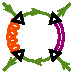
\includegraphics{qcd/diagrams/QCD-4qFlow2.pdf}\end{gathered}+\ldots
+\frac{1}{2}\,\begin{gathered}\includegraphics{qcd/diagrams/QCD-4qFlow3.pdf}\end{gathered}+\ldots
\Bigg)\,,\label{eq:qcd4fermiFlowHad}
\end{align}
where the diagrams $\propto\lambda_{\psi,k}^2$ and $\propto\lambda_{\psi,k}\alpha_{s,k}$ from \cref{eq:qcd4fermiFlowHad} vanish due to the hadronization constraint \eqref{eq:qcd4fzero}.
Further details and explicit flow equations can be found in Sec.~III.E  and the corresponding App.~L of \nbccite{FuQCD}.

This complete bosonization of the four-fermi coupling entails, that the complete dynamics of the $\sigma-\pi$ channel is encoded using the effective hadronic composites.
The emergent four-fermi coupling is on a computational level completely replaced by the Yukawa-type interaction of $\Lqbqphi$ from \cref{eq:qcdLqbqphi}, with multi scatterings of the resonant channel encoded in the effective potential $\LpotExpI$ of \cref{eq:qcdLpot}.
$\LpotExpI$ is directly related to the equilibrium thermodynamic grand potential density $\Omega$, see \cref{eq:thermalGrandPotentialDensity} of \cref{app:grandCanonicalPartitionFunction} and Sec.~III.F of \nbccite{FuQCD} for specifics. 
$\LpotExpI$ is the central quantity used to study \csb{} and the confinement-deconfinement transition.\bigskip

\fullWidthTwoColumnSubFigures%
	[!t] % Placement
	{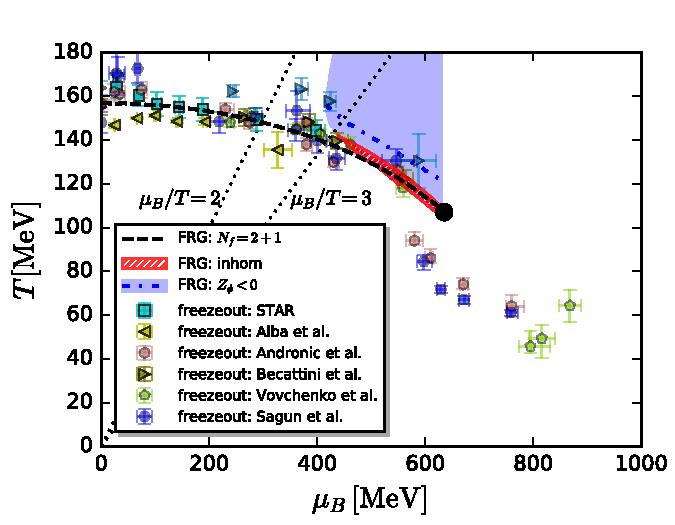
\includegraphics[width=\subcaptionFigureWidth]{qcd/figures/PhysRevD.101.054032Fig21noType3.pdf}} % left figure
	{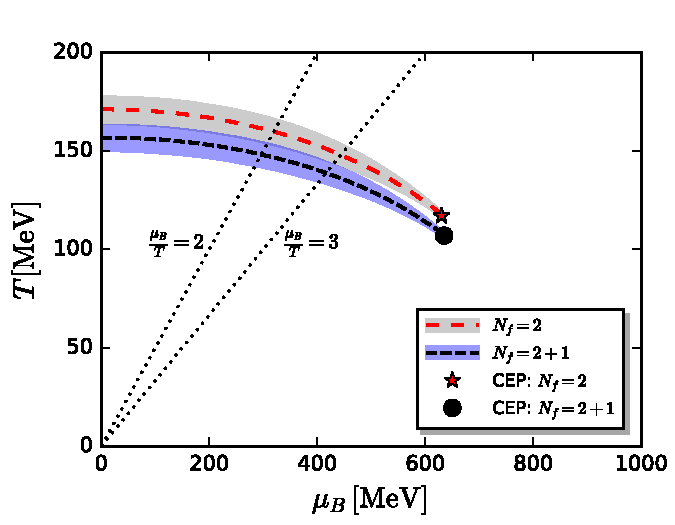
\includegraphics[width=\subcaptionFigureWidth]{qcd/figures/PhysRevD.101.054032Fig20noType3.pdf}} % Right figure
	[fig:fuQCDpd,fig:fuQCDpd2]
	{%
		Phase diagram of $N_f=2+1$ flavor \qcd{} including experimental freeze-out data~\cite{\qcdExpFreezeout} on the left \subref{fig:fuQCDpd} and $N_f=2$ and $2+1$ flavor \qcd{} phase diagram on the right \subref{fig:fuQCDpd2}.
		Information about the resulting and underlying (physical) parameters can be found in Tab.~I of \nbccite{Fu:2019hdw}.
		The red and blue regions on the left \subref{fig:fuQCDpd} are related to the possible emergence of inhomogeneous phases and are discussed in detail in \cref{subsec:inhomoLiterature}.
		The bands and dotted lines on the right \subref{fig:fuQCDpd2} mark the crossover region on temperature for the chiral condensate.
		An augmented version of the left figure \subref{fig:fuQCDpd} can be found in Fig. 13 of \ccite{Gao:2020qsj}, including lattice data~\cite{Boucaud:2018xup,Borsanyi:2020fev}, \dses{} results~\cite{Fischer:2014ata,Gao:2015kea}, and of course the results of \ccite{Gao:2020qsj} itself.
		\textit{Taken from the arXiv source for Fig. 21 and 20 of \ccite{Fu:2019hdw}.
		\ccbysaLicense{W.-j. Fu}}
	}%
	{fig:fuQCDpds}
At this point we want to comment and present one of the central results of \ccite{Fu:2019hdw}, the phase diagram of $N_f=2+1$ and $N_f=2$ flavor \qcd{} in \cref{fig:fuQCDpds} with realistic quark/pion masses and decay constants $f_\pi$ and $f_K$.
These phase diagrams must be considered seminal results and represent the culmination of a massive research effort by large parts of the \frg{} community towards such first principle results for \qcd{}.

The phase diagrams are computed up to $\mu_B/T\approx 6$ and include the chiral crossover transition between a \hbp{} at low temperatures and an approximately \symp{} at high temperatures.
The chiral crossover transition ends in a \cep{}.
Note that due to non-vanishing quark masses chiral symmetry only gets approximately restored and the transition is a smooth crossover instead of a second-order phase transition, which is found in the chiral limit.
The crossover temperatures at vanishing $\mu_B$ are found to be
\begin{align}
	T_{c,{\scriptscriptstyle{N_f=2}}}=171\,\MeV\,,\qquad T_{c,{\scriptscriptstyle{N_f=2+1}}} = 156\,\MeV\,,\label{eq:TC0qcd}
\end{align}
with a curvature $\kappa$ of the phase boundary $T_c(\mu_B)$ of
\begin{align}
	\kappa_{\scriptscriptstyle{N_f=2}}=0.0176(1)\,,\qquad \kappa_{\scriptscriptstyle{N_f=2+1}}=0.0142(2)\,,\label{eq:kappaQCD}
\end{align}
as the quadratic expansion coefficient of $T_c(\mu_B)$ around $\mu_B=0$:
\begin{align}
	\frac{T_c(\mu_B)}{T_c}&=1-\kappa \left(\frac{\mu_B}{T_c}\right)^2+\cdots\,.\label{eq:kappaTc}
\end{align}
The \ceps{} are located at
\begin{subequations}\label{eq:cepqcd}
\begin{alignat}{2}
	&(T_,\vts \mu_B)_{\scriptscriptstyle{\text{CEP},N_f=2}} &&= (117, 630)\,\MeV\,,\label{eq:cep2qcd}\\
	&(T_,\vts \mu_B)_{\scriptscriptstyle{\text{CEP},N_f=2+1}} &&= (107, 635)\,\MeV\,,\label{eq:cep3qcd}
\end{alignat}
\end{subequations}
which entails
\begin{subequations}\label{eq:zcepqcd}
\begin{alignat}{2}
	&(T/{\mu_B})_{\scriptscriptstyle{\text{CEP},N_f=2}} &&= 5.38\,,\label{eq:zcep2qcd}\\
	&(T/{\mu_B})_{\scriptscriptstyle{\text{CEP},N_f=2+1}} &&= 5.93\,.\label{eq:zcep3qcd}
\end{alignat}
\end{subequations}
A discussion of these results (and the values themselves) can be found in Sec.~V.D \dash{} Eqs.~(121)\dash{}(127) \dash{} of \ccite{Fu:2019hdw}.
Since we are primarily working with quark chemical potential $\mu$: note that $\mu_B=3\mu$ and thus $\kappa\rightarrow 9\kappa\equiv \kappa'$, \ie{}, $\kappa'_{\scriptscriptstyle{N_f=2}}=0.1584(9)$ in terms of $\mu$ instead of $\mu_B$ in \cref{eq:kappaQCD}.

The indication for inhomogeneous phases in \cref{fig:fuQCDpd} will be discussed in \cref{subsec:inhomoLiterature}.
The limitation of the results in \ccite{Fu:2019hdw} to $\mu_B/T\smallerlesssim 6$ has several reasons. 
One is the inclusion of only the scalar-pseudoscalar $\sigma-\pi$ channel \dash{} a discussion with qualitative and quantitative predictive power at $\mu_B/T \smallergtrsim 6$ should include at least the dominant diquark and vector-meson channels.
Another technical limitation of \ccite{Fu:2019hdw} is the application of a \frg{} Taylor expansion, \cf{} \teRef{}, for the effective potential $\LpotExpI$. 
A study of non-smooth, potentially first-order, chiral phase transitions requires \dash{} as we will argue throughout this work \dash{} proper shock capturing schemes for the underlying \pdes{}, \cf{} \ccite{Grossi:2019urj,zerod1,zerod2,zerod3,Ihssen2020,Grossi:2021ksl,Stoll:2021ori,Ihssen:2022xkr,Ihssen:2023xlp} and \cref{subsec:RGflow} as well as \cref{chap:zeroONSU2,chap:GN}.
In the context of \ccite{Fu:2019hdw} especially the recent work~\cite{Ihssen:2023xlp} represents significant progress in terms of an application of the recently developed \cfd{} perspective for \frg{} flow equations.

\FloatBarrier
\paragraph{Sequential decoupling and the emergence of NJL-/QMM-type LEFTs from QCD}\phantomsection\label{paragraph:qcdDec}\mbox{}\\%
\fullWidthTwoColumnSubFigures%
	[!t] % Placement
	{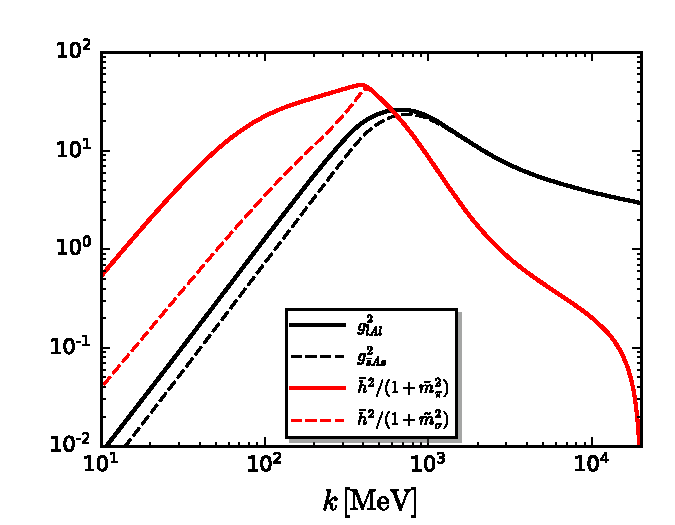
\includegraphics[width=\subcaptionFigureWidth]{qcd/figures/PhysRevD.101.054032Fig18noType3.pdf}} % left figure
	{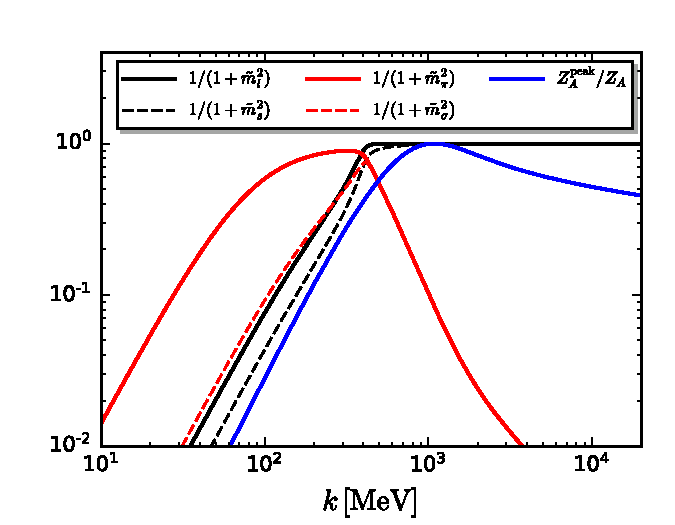
\includegraphics[width=\subcaptionFigureWidth]{qcd/figures/PhysRevD.101.054032Fig19noType3.pdf}} % Right figure
	[fig:fuQCDgh,fig:fuQCDgaps]
	{%
		Dimensionless four-quark single gluon couplings (in black) and dimensionless four-quark single meson exchange couplings (red) on the left \subref{fig:fuQCDgh} and
		dimensionless propagator gaps for quarks (in black), mesons (in red), and a gluon dressing function for comparison (in blue) on the right \subref{fig:fuQCDgaps}.
		\textit{Taken from the arXiv source for Fig. 18 and 19 of \ccite{Fu:2019hdw}.}
		\ccbysaLicense{W.-j. Fu}
	}%
	{fig:fuQCDdecoupling}
One extremely interesting and for our work relevant observation in \ccite{Fu:2019hdw} is the observed \textit{sequential decoupling of dynamic, relevant degrees of freedom} during \rgscale-evolution from the \uv{} towards the \ir{}.
The phenomenon is visualized in \cref{fig:fuQCDdecoupling} and described at length in Sec.~V.D of \ccite{Fu:2019hdw}.
We will give a concise summary here using \cref{fig:fuQCDdecoupling}.

\Cref{fig:fuQCDgh} includes dimensionless quark-gluon couplings and dimensionless quark-meson couplings and we can observe, that the quark-gluon coupling dominates in the \uv{} for scales 
$k\smallergtrsim 1\,\GeV$.
In turn, for scales $k\smallerlesssim 1\,\GeV$, the quark-meson couplings gain importance and become dominant at $k\approx 0.6\,\GeV$, while the quark-gluon couplings decay rapidly \dash{} note the logarithmic scale on the vertical axis of \cref{fig:fuQCDgh}.
This observation is further supported by considering the propagator gappings in \cref{fig:fuQCDgaps}: the gluons decouple first only followed by the quarks and mesons.
First the gluonic dynamics decouples from the matter sector, followed by the quark- and \sigmaModes{} and ultimately the pion decouples last.
Note the dominance of pions for the dynamics at low \rgscales{} $k\approx 0.2\,\GeV$.
The connection and emergence of chiral perturbation theory in vacuum in this context is discussed in \ccite{Eser:2018jqo,Divotgey:2019xea,Eser:2019pvd}.
We will discuss the dynamics of such pionic modes in comparison to radial \sigmaModes{} at length in our study of zero-dimensional $O(N)$ models in \cref{subsec:0dONresults}.
The discussion of the interplay of bosonic and fermionic fluctuations is at the heart of our study of the \gn{} model at finite $N$ in \cref{subsec:gnyFiniteNresults} and we observe a similar decoupling hierarchy between fermionic and bosonic modes in this low-dimensional model.

This sequential decoupling of dynamic/relevant degrees of freedom gives rise to an intriguing and for the \frg{} practitioners extremely attractive point of view: first principle \frg{} \qcd{} computations~\cite{Fu:2019hdw} show, that the highly complicated and involved gauge-dynamics of \qcd{} decouples for low \rgscales{} $k\approx 1\,\GeV$. 
Furthermore, by employing dynamic hadronization, we observe the emergence of Polyakov loop enhanced \loefts{}, see, \eg{}, \ccite{Braun:2015fva,Schaefer:2007pw,Haas:2013qwp}.
With the currently discussed hadronization prescription, \viz{} the \pqmm{} emerges.
The relevant dynamic degrees of freedom, \viz{} quarks and mesons (as quark-anti-quark composites), and their interactions at $k\smallerlesssim1\,\GeV$ are properly captured by \loefts{} like the \pqmm{}.
Studies like \ccite{Fu:2019hdw} allow for \textit{QCD-assisted} \loefts{}: using full fledged, first principle \frg{} computations for \qcd{} to initialize \loefts{} like the \pqmm{} at scales $k\smallerlesssim 1\,\GeV$.
Typically such theories have been used as low-energy effective models by fitting vacuum observables to determine model parameters, \cf{} \cref{sec:cdwmf} and, \eg{}, \ccite{Schaefer:2007pw}.
The maturing \frg{} computations for \qcd{} can be used to eliminate the need for such parameter fits by providing input for the model parameters from first principle \qcd{} flows.
Thus promoting them from \textit{``mere effective models''} to \textit{QCD-assisted} \loefts{}.
First steps of such improvements can be found in \ccite{Haas:2013qwp,Herbst:2013ufa,Springer2017} and the more recent works~\cite{Leonhardt:2019fua,Ihssen:2023xlp}.

\subsubsection{The quark-meson model}\label{subsubsec:qcdQMM}
We want to conclude our introduction into \qcd{} and \loefts{} by actually introducing the \loeft{} we will be using in \cref{chap:QMM}: the \acrrepeatEmph{qm} model, sometimes also referred to as linear-$\sigma$ model. 
The \qmm{} and variants/extensions of it \dash{} including the \pqmm{} \dash{} are incredibly popular in the field of theoretical \hep{}.
An extensive review of the vast literature regarding the model is beyond the scope of the current work.
At this point we only want to reference the very incomplete list of \qmm{} \frg{} literature~\cite{Ellwanger:1994wy,Schaefer:2004en,Rennecke:2016tkm,Fu:2018qsk,Alkofer:2018guy,Tripolt:2017zgc,Eser:2018jqo,Divotgey:2019xea,Eser:2019pvd,Grossi:2021ksl,Ihssen:2023xlp}.
For a review of primarily mean-field/large-$N_c$ results we refer to \ccite{Scadron:2013vba} and for a review of \frg{} studies with the \qmm{} we refer to Sec.~III.B of \nbccite{Fu:2022gou}.
Additional/complementary references to the ones provided in \ccite{Fu:2022gou} may be found in the last line of the fourth-to-last paragraph of Sec.~V.C of \nbccite{Fu:2019hdw}.\bigskip

In this work we consider the $N_f=2$ flavor \qmm{}, which in the present context, emerges as the part of \cref{eq:GammaQCD} relevant for the dynamics at low \rgscales{} $k\smallerlesssim 1\,\GeV$.
The \qmm{} is formed by $\mathcal{L}_{\MFpsib\MFpsi}[\mkern1.5mu{}\xcancel{\MFA}\mkern1.5mu{},\MFpsi,\MFpsib\mkern0.5mu{}]$, $\Lqbqphi$, $\LphiKin$, and $\mathcal{L}_{V}[\mkern1.5mu{}\xcancel{A}\mkern1.5mu{},\MFphi]$ from \cref{eq:qcdLqbqKi,eq:qcdLqbqphi,eq:qcdLphiKin,eq:qcdLpot}.
We will consider it primarily in \lpa{}, \cf{} \deRef{}, and without considering the statistical confinement provided by the Polyakov loop potential.
To get specific, we study the following \eaa{},
\begin{align}
\FSeaa_k^\mathrm{QMM}[\FSmf{\FSsf}]\equiv \intx[x]\,\bigg( 
\MFpsib(\gamma_\mu \partial_\mu -\gamma_4\mu + h \MFphi_i \uIItv^{i} )\MFpsi
+\frac{1}{2}\big(\partial_\mu\MFphi\big)^2
+U_{k}(\MFrho)
\bigg)\,,
\label{eq:QMMeaa}
\end{align}
with the field-independent, constant Yukawa coupling $h$ and the scale-dependent mesonic self-interaction potential $U_k(\MFrho)$ as a function of the $O(4)$ invariant $\MFrho\equiv\frac{1}{2}\MFphi^2$. 
In $\FSmf{\FSsf}\equiv(\MFphi,\MFpsi,\MFpsib)$ we consider four dynamic, on this level fundamental, mesons $\MFphi=\langle\Fphi\rangle\equiv (\MFphi_0,\pi_1,\pi_2,\pi_3)$ and $N_c=3$ dynamic quarks $\MFpsi=\langle\Fpsi\vts\rangle$ and $\MFpsib=\langle\Fpsib\vts\rangle$ with $N_f=2$ flavors.

The \qmm{} \dash{} its \eaa{} \eqref{eq:QMMeaa} in \lpa{} \dash{} shares the chiral symmetry
\begin{align}
SU(2)_{\suL}\otimes SU(2)_{\suR}\otimes U(1)_{\suV} \simeq SU(2)_{\suV}\otimes SU(2)_{\suA}\otimes U(1)_{\suV}
\label{eq:QMMchiral}
\end{align}
with \qcd{}, see \cref{paragraph:qcdChiral}.
The model, especially in the context of a \textit{QCD-assisted} \loeft{}, is ideally suited to study the dynamics of \csb{}.
For the mesons chiral symmetry manifests through the equivalence $SU(2)_{\suL}\otimes SU(2)_{\suR} \simeq SO(4)$ as an $SO(4)$ symmetry, which motivates the $O(4)$ vector
\begin{align}
\MFphi \equiv (\varphi_0,\pi_1,\pi_2,\pi_3)\,,
\label{eq:phiVector}
\end{align}
with the $1^-(0^-)$ isovector, pseudoscalar pions\footnote{%
	Note that we are referring here to flavor eigenstates with $(\pi_1,\pi_2,\pi_3)$.
	The charge eigenstates $\pi_\pm$ and $\pi_0$ can be obtained in the usual manner $\pi_\pm=(\pi_1\mp \iu \pi_2)/\sqrt{2}$ and $\pi_{0}=\pi_3$.
} and the $0^+(0^+)$ isoscalar, scalar $\MFphi_0$/$\sigma$\footnote{
	We reserve the symbol $\sigma$ in equations and expressions for the value we evaluate $\MFphi_0$ on, \ie{}, the possible solution of $\MFphi_{0;\eom}\equiv\sigma$ we probe for.
	This distinction will become clearer with the applications in the main part of this thesis in \cref{chap:zeroONSU2,chap:GN,chap:QMM}.
	In the text we will usually refer to the zeroth component of $\MFphi$ as radial, massive, or \sigmaMode{} depending on the context.
}.
The pions are in the isospin triplet $SU(2)_\suV\simeq SO(3)$ and are the Nambu-Goldstone bosons of the $SU(2)_\suA$ chiral symmetry breaking, which manifests in the mesonic sector as a breakdown of $SO(4)$ to $SO(3)$ with the radial $\MFphi_0$ as massive \sigmaMode{}.

We will reserve further discussions for the applications in \cref{chap:QMM} apart from one last remark at this point regarding $U(1)_\suA$ symmetry in the $N_f=2$ \qmm{}.
For $N_f=2+1$ flavors the anomalous $U(1)_\suA$ symmetry breaking, mentioned in \cref{paragraph:qcdChiral}, is usually included in the three flavor \qmm{} by means of a t'Hooft determinant~\cite{tHooft:1976rip}, see, \eg{}, \ccite{Schaefer:2008hk,Scadron:2013vba,Rennecke:2015lur,Rennecke:2016tkm,Braun:2018bik}.
It is a determinant in flavor space resulting in a six-point interaction and it is crucial to properly reproduce the aforementioned $\eta-\eta'$ mixing~\cite{Kobayashi:1970ji,Kobayashi:1971qz,DelDebbio:2004ns,Luscher:2010ik,Ce:2014sfa}.
In the $N_f=2$ case such a determinant manifests, in terms of quark-anti-quark bilinears, as an ordinary four-fermi coupling
\begin{align}
 \mathcal{O}^{(S+P)_{-}}_{ijlm}{\MFpsib}_i\MFpsi_j{\MFpsib}_l\MFpsi_m=&(\MFpsib\,t^0 \MFpsi)^2+(\MFpsib\,\gammach t^0 \MFpsi)^2 -(\MFpsib\,t^a \MFpsi)^2-(\MFpsib\,\gammach t^a \MFpsi)^2\,,\label{eq:QMMSpPm}
\end{align}
where we adapted the notation of App.~B of \nbccite{Fu:2022gou}.
The $N_f=2$ \qmm{} is constructed (in terms of Fierz-complete couplings) by the linear combination (sum) of \cref{eq:QMMSpPm} with the $U(1)_\suA$-symmetric channel
\begin{align}
 \mathcal{O}^{(S-P)_{+}}_{ijlm}{\MFpsib}_i\MFpsi_j{\MFpsib}_l\MFpsi_m=&(\MFpsib\,t^0 \MFpsi)^2-(\MFpsib\,\gammach t^0 \MFpsi)^2+(\MFpsib\,t^a \MFpsi)^2-(\MFpsib\,\gammach t^a \MFpsi)^2\,\label{eq:QMMSmPp}\, .
\end{align}
Such a linear combination completely eliminates/decouples the three $1^-(0^+)$ isovector, scalars $\MFpsib\,t^a \MFpsi$ and the $0^+(0^-)$ isoscalar, pseudoscalar $\MFpsib\,\gammach t^0 \MFpsi$ as the chiral partners of the pions and $\sigma$.
In that sense $U(1)_\suA$ is ``maximally broken'' in the $N_f=2$ flavor \qmm{}~\cite{Rennecke:2015lur}.
Phenomenologically these chiral partners correspond to the heavy $a_0$ and $\eta_N$ mesons \dash{} with $m_{a_0}\approx 980\,\MeV$~\cite{ParticleDataGroup2022Aug} and $\eta_N$ not really observable (only as a mixture/part of $\eta$/$\eta'$).
For the dynamics of $N_f=2$ \csb{} those heavy partners are not relevant and are thus usually not considered in the $N_f=2$ \qmm{}.